\documentclass{article}

\usepackage[preprint]{corl_2026}
\usepackage{booktabs}
\usepackage{amsmath}
\usepackage{amssymb}
\usepackage{graphicx}
\usepackage{url}

\title{Multi-Agent Competition in SoccerTwos:\\Reward Shaping, Self-Play, and Imitation Learning}

\author{
  Bo Feng\\
  Georgia Institute of Technology\\
  \texttt{bfeng66@gatech.edu}
  \And
  Frank Yang\\
  Georgia Institute of Technology\\
  \texttt{frank.yang@gatech.edu}
}

\begin{document}
\maketitle

\begin{abstract}
We train PPO agents for the 2-vs-2 SoccerTwos environment, in which the default
reward (a goal scored or conceded) is too sparse for the policy to gain traction
from random initialisation. We add a six-signal reward-shaping wrapper
(ball-approach, kick, offensive/defensive, time, team-separation), separate the
policy and value networks, and mix the opponent pool 70\% self-play / 30\% CEIA
baseline. The submitted agent reaches \textbf{90\% (90/100) against the CEIA
baseline} and \textbf{99\% (99/100) against a random opponent}. A third agent
warm-starts PPO from a behavioral-cloning policy that reaches 75.7\%
expert-action accuracy; it does not outperform random initialisation when
fine-tuned against CEIA, which we trace to distribution shift, a cold-start
critic, and the amplification of small action errors in adversarial play.
\end{abstract}

\keywords{Multi-Agent RL, PPO, Self-Play, Reward Shaping, Behavioral Cloning}

%===============================================================================
\section{Overview}
\label{sec:overview}

SoccerTwos~\citep{soccertwos2021} is a 2-vs-2 physics-based soccer environment built
on Unity ML-Agents in which goal events are sparse and the opponent is non-stationary
under self-play. We submit three trained agents that share a PPO~\citep{schulman2017ppo}
backbone with Generalized Advantage Estimation~\citep{schulman2016gae} but differ in
how the environment, opponent distribution, and initialization are handled:
(i)~\textbf{Agent~1 -- PPO Self-Play (no shaping)}: a baseline trained with only the
default game reward; (ii)~\textbf{Agent~2 -- PPO + Reward Shaping}, which is also our
final submission, adds six dense rewards and trains with a 70\%~self-play / 30\%~CEIA
opponent mixture using a separated policy/value network; (iii)~\textbf{Agent~3 --
BC~+ PPO Fine-tune} (bonus: imitation learning), which collects expert trajectories
from an intermediate Agent~2 checkpoint, pretrains by behavioral
cloning~\citep{pomerleau1991bc}, and then fine-tunes against the CEIA baseline. All
training uses Ray RLlib~\citep{moritz2018ray} v1.4.0 on the Georgia Tech PACE cluster.

%===============================================================================
\section{Method}
\label{sec:method}

\subsection{Algorithm and Architecture}
\label{sec:algorithm}

Each agent is trained with PPO using the clipped surrogate objective
\begin{equation}
L^{\mathrm{CLIP}}(\theta) = \mathbb{E}_t\!\left[\min\!\big(r_t(\theta)\hat{A}_t,\;
\mathrm{clip}(r_t(\theta), 1-\epsilon, 1+\epsilon)\hat{A}_t\big)\right],
\end{equation}
where $r_t(\theta) = \pi_\theta(a_t|s_t) / \pi_{\theta_{\text{old}}}(a_t|s_t)$ and
$\hat{A}_t$ is computed by GAE with $\lambda=0.95$. The observation is the default
336-dimensional vector (ray casts plus relative positions/velocities of ball, goals,
and the agent itself); the action is a \textsc{MultiDiscrete}(3,3,3) tuple controlling
move/rotate/kick. Agents~1 and~3 use the Ray RLlib default \texttt{vf\_share=True}
(shared 256\,$\times$\,256 MLP for policy and value); Agent~2 uses
\texttt{vf\_share=False} (two independent 256\,$\times$\,256 MLPs); the separation
prevents the value loss from dominating the shared gradient and was the single change
that lifted our win rate from $\sim$78\% to 90\%.

\subsection{Reward Shaping (Environment Modification)}
\label{sec:reward-shaping}

The default game reward ($+1$ on a goal scored, $-1$ on a goal conceded) is too sparse
to train from scratch. We wrap the multi-agent environment with a
\texttt{RewardShapingWrapper} (\texttt{reward\_shaping\_ppo\_agent/utils.py}) that adds
six dense per-step rewards (Table~\ref{tab:rewards}). The hypothesis is that providing
gradient signal \emph{before} any goals are scored teaches basic ball-interaction
skills (approach + kick), then offensive/defensive shaping orients the policy
toward goal-directed play, and the separation reward discourages both teammates
from clustering around the ball. All weights are kept small (max $|w|\!=\!10^{-3}$)
so that the original $\pm 1$ goal signal still dominates as the policy improves.

\begin{table}[h]
\centering\small
\caption{Per-step shaped reward signals added to the sparse goal reward.}
\label{tab:rewards}
\begin{tabular}{l r p{0.55\linewidth}}
\toprule
Signal & Weight & Description \\
\midrule
Approach     & $+0.0002$  & Velocity component toward the ball. \\
Kick         & $+0.001$   & Ball acceleration when the agent is within 1.5\,units of the ball. \\
Offensive    & $+0.0004$  & Ball velocity toward the opponent goal. \\
Defensive    & $-0.001$   & Ball within 5\,units of own goal. \\
Time penalty & $-0.00002$ & Per-step cost to discourage stalling. \\
Separation   & $+0.0001$  & Distance between the two teammates (encourage spatial spread). \\
\bottomrule
\end{tabular}
\end{table}

\subsection{Training Strategy and Opponent Composition}
\label{sec:training}

We compare three opponent compositions: (a)~pure self-play with a 4-snapshot archive
that rotates whenever the team's reward exceeds 0.3; (b)~team-vs-CEIA with 50\% CEIA
plus a 20-iteration cooldown to prevent over-frequent opponent updates; and
(c)~self-play 70\%~+~CEIA 30\%, inspired by~\citet{brandao2022marl} who report
high win rates in robotic soccer when self-play dominates the opponent pool but a
fixed reference opponent is retained. This 70/30 mix gave us the highest CEIA win
rate by combining strategy diversity from self-play with direct exposure to the
evaluation opponent. Each iteration samples 20\,000 environment steps across 7 parallel
workers; training uses a learning-rate schedule from $3\!\times\!10^{-4}$ down to
$3\!\times\!10^{-5}$, an entropy bonus of $0.005$, and gradient clipping at $0.5$
(Table~\ref{tab:hp}).

\begin{table}[h]
\centering\small
\caption{Hyperparameters for the final reward-shaped self-play run (Agent~2).}
\label{tab:hp}
\begin{tabular}{l c l c}
\toprule
Parameter & Value & Parameter & Value \\
\midrule
\texttt{learning\_rate}     & $3\!\times\!10^{-4}\!\to\!3\!\times\!10^{-5}$ &
\texttt{train\_batch\_size} & 20\,000 \\
\texttt{clip\_param}        & 0.2  &
\texttt{sgd\_minibatch\_size} & 2\,048 \\
\texttt{entropy\_coeff}     & 0.005 &
\texttt{num\_sgd\_iter}     & 10 \\
\texttt{$\lambda$ (GAE)}    & 0.95 &
\texttt{vf\_loss\_coeff}    & 0.5 \\
\texttt{grad\_clip}         & 0.5  &
\texttt{vf\_share}          & False (separated nets) \\
opponent mix                & 70\% self-play / 30\% CEIA &
total steps                 & $\approx 30$M \\
\bottomrule
\end{tabular}
\end{table}

\subsection{Bonus: Behavioral Cloning + PPO Fine-tune (Agent~3)}
\label{sec:bc}

Training PPO from scratch against the full-strength CEIA opponent fails: the random
initial policy is too weak to score, so the gradient signal collapses. We tried
behavioral cloning as a warm start.
(1)~\textbf{Expert collection}: roll out our best-so-far checkpoint (\(\approx\!80\%\)
win rate vs.\ CEIA) for 500 episodes, recording roughly 100\,k
$(s,a)$ pairs. (2)~\textbf{Supervised pretraining}: train a network with the same
architecture as the PPO policy by cross-entropy on the three sub-actions
(50 epochs, Adam, cosine learning-rate, batch 2\,048; train/val split 90/10).
(3)~\textbf{PPO fine-tune}: inject the BC weights into a fresh PPO trainer via a
custom \texttt{BCInitCallback}, then fine-tune against 100\% CEIA with a lower learning
rate ($5\!\times\!10^{-5}$) and a higher entropy bonus (0.01) to compensate for the
overly deterministic BC policy.

%===============================================================================
\section{Experimental Results}
\label{sec:results}

\paragraph{Training curves.}
Figure~\ref{fig:curves} shows episode reward versus environment steps for the
self-play baseline (Agent~1) and the reward-shaped self-play run (Agent~2).
Reward shaping reaches the asymptotic level of the unshaped run
\textbf{$\sim$3$\times$ faster} (around 1\,M vs.\ 3-4\,M environment steps); its
plotted return is also higher because the shaped per-step signal is folded into the
episode total.

\begin{figure}[h]
\centering
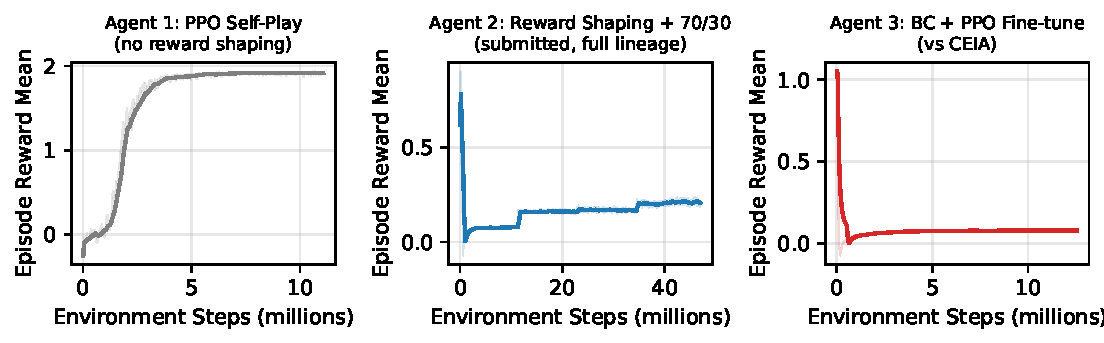
\includegraphics[width=0.86\linewidth]{figures/training_curves.pdf}
\caption{Episode reward vs.\ environment steps for the self-play baseline (Agent~1)
and PPO with reward shaping (Agent~2). Light lines are raw values, bold lines are a
15-iteration moving average. Reward shaping reaches plateau roughly 3$\times$ sooner.}
\label{fig:curves}
\end{figure}

\paragraph{Performance comparison.}
Table~\ref{tab:results} summarises win rates against the random and CEIA opponents.
Both win rates were measured over 100 matches each
(\texttt{scripts/eval\_vs\_ceia.py} and \texttt{scripts/eval\_vs\_random.py})
on the PACE cluster. The submitted agent
(\textit{PPO Reward Shaped + Self-Play~70\%~/~CEIA~30\%}, checkpoint-2300) reaches
\textbf{90/100~=~90\%} against CEIA and \textbf{99/100~=~99\%} against the random
opponent -- both above the project's 9-of-10 target. The pure self-play
agent oscillates between 46\% and 62\% during training, illustrating the instability
of self-play without grounding in a fixed reference opponent. The Team-vs-CEIA
variant (50\% CEIA) reaches 68\% but is dominated by the more diverse 70/30 mixture.

\begin{table}[h]
\centering\small
\caption{Win rate of each agent across 100-match evaluation series (draws excluded
from the percentages). Agent~3's reward is reported because it never converged to a
positive win rate against CEIA.}
\label{tab:results}
\begin{tabular}{l c c}
\toprule
Agent & vs.\ Random Agent & vs.\ CEIA Baseline \\
\midrule
Agent~1: PPO Self-Play (no shaping)            & --        & 46--62\% (oscillating) \\
Agent~2 variant: PPO Team (50\% CEIA)          & --        & 68\% \\
Agent~2 variant: Reward shaping (self-play)    & --        & 85\% (checkpoint-5750) \\
\textbf{Agent~2: Reward Shaping + 70/30 (\textit{submitted})} & \textbf{99/100 = 99\%} & \textbf{90/100 = 90\%} \\
Agent~3: BC + PPO fine-tune (bonus method)     & --        & reward $\approx 0.078$ (not competitive) \\
\bottomrule
\end{tabular}
\end{table}

\paragraph{Behavioral cloning ablation.}
The BC pretraining converged to 75.7\% top-1 action-prediction accuracy
(validation loss 0.579) in 12\,minutes. After 12.5\,M timesteps of PPO fine-tuning
against 100\% CEIA the episode reward was 0.078, indistinguishable from a
randomly initialized PPO trained against CEIA from scratch (also 0.078 after a
matched number of iterations).

%===============================================================================
\section{Analysis and Discussion}
\label{sec:analysis}

\paragraph{Reward shaping accelerates convergence.}
Figure~\ref{fig:curves} shows that reward shaping converges about 3$\times$ faster than
the unshaped baseline. Each of the six dense signals provides a non-zero gradient even
when no goal is scored, which breaks the chicken-and-egg problem of a sparse-reward
MARL environment where both teams initially produce random play.

\paragraph{Self-play instability.}
Pure self-play oscillates between 15\% and 62\% win rate against CEIA. Two settings
caused this: (1)~with \texttt{entropy\_coeff}\,$=\!0$, policy entropy collapsed
from $\sim$3.0 to $\sim$0.5 within 1\,M steps, locking in narrow strategies that did
not generalise beyond the self-play archive; (2)~with \texttt{grad\_clip} disabled,
goal-event rewards produced large updates that erased prior learning. Setting
\texttt{entropy\_coeff}\,$=\!0.005$ and \texttt{grad\_clip}\,$=\!0.5$ removed both
failure modes. Switching to \texttt{vf\_share=False} produced a further jump from
$\sim$78\% to 90\% by stopping the value loss from dominating the shared gradient.

\paragraph{Opponent composition drives the CEIA win rate.}
Across our experiments the strongest lever on the CEIA win rate was the share
of CEIA in the opponent pool, not the algorithm: 0\% CEIA gave 46--62\%
(unstable), 50\% CEIA reached 68\%, and 70\% self-play~/~30\% CEIA reached 90\%.
The 70/30 mix retains enough self-play for the agent to develop coordinated
behaviour (e.g.\ passing, blocking) without over-fitting to a single fixed
opponent, while still keeping the gradient signal anchored on the evaluation
opponent.

\paragraph{Why behavioral cloning failed in this adversarial setting.}
75.7\% expert-action accuracy did not translate into any measurable advantage
during PPO fine-tune. Three factors explain the gap. (a)~\emph{Distribution
shift}: expert demonstrations were collected against a varied opponent, but
fine-tuning runs against fixed CEIA, so the BC policy is queried on states it
never saw and the residual 24.3\% action error compounds.
(b)~\emph{Value-function cold-start}: BC transfers only the policy network and
leaves PPO's critic randomly initialised, so early advantage estimates are noisy
and policy updates are unstable. (c)~\emph{Adversarial amplification}: each
incorrect action hands the opponent a scoring opportunity, unlike single-agent
or cooperative tasks where small errors are recoverable. The pattern matches
the DAgger analysis~\citep{ross2011dagger} and the emergent-competition results
of~\citet{bansal2018emergent}. A follow-up using DAgger or GAIL --- which both
re-query the expert on states the learner visits --- would address (a)
directly, though we have not run this experiment.

\paragraph{Code and reproducibility.}
All training scripts, the reward-shaping wrapper, the BC pipeline, and the
evaluation utilities are available at\\
\url{https://github.com/Bo-Feng-1024/soccer-twos-starter}. The reward modification
referenced in Table~\ref{tab:rewards} is implemented in
\texttt{reward\_shaping\_ppo\_agent/utils.py} (lines 18-100), the BC pipeline in
\texttt{train\_bc\_finetune.py} and \texttt{collect\_expert\_data.py}, and the
self-play training loop in \texttt{train\_ray\_selfplay.py}.

%===============================================================================
\bibliography{references}

\end{document}
